\documentclass[aps,prb,superscriptaddress,nofootinbib]{revtex4}
\usepackage{amsfonts}
\usepackage{amsmath}
\usepackage{amssymb}
\usepackage{graphbox}
\usepackage{graphicx}
\usepackage{caption}
\usepackage{bm}
\usepackage{bbm}
\usepackage{cancel}
\usepackage{color}
\usepackage{mathrsfs}
\usepackage[colorlinks,bookmarks=true,citecolor=blue,linkcolor=red,urlcolor=blue]{hyperref}
\usepackage{simpler-wick}
\usepackage{appendix}
\usepackage{float}
\usepackage{array}
\usepackage{booktabs}
\usepackage[export]{adjustbox}
\setlength{\parindent}{10 pt}
\setlength{\parskip}{2 pt}
\setcounter{MaxMatrixCols}{30}
\bibliographystyle{apsrev}
\newcommand{\RNum}[1]{\uppercase\expandafter{\romannumeral #1\relax}}
\newcommand{\normord}[1]{{:\mathrel{#1}:}}
\def\tbs{\textbackslash}
\def \tr{\operatorname{tr}}
\def \Tr{\operatorname{Tr}}


\begin{document}
\title{Luttinger Liquid}
\author{Jie Ren}


\maketitle


\tableofcontents

\section{Bosonization}

\subsection{1D free massless fields}
\paragraph*{Bosonic fields}
Consider the massless scalar field $H_B = \frac{1}{2}\int dx[\Pi^2+(\partial_x\phi)^2]$, where the field $\phi$ and momentum $\Pi$ obey the canonical commutation relation $[\phi(x),\Pi(y)] = i\delta(x-y)$.
The operator expansions for $\phi$ and $\Pi$ are:
\begin{equation*}
	\phi(x) = \int \frac{dp}{2\pi} \frac{1}{\sqrt{2|p|}} e^{-\frac{1}{2}\alpha|p|} \left[a_p e^{ipx} + a_p^\dagger e^{-ipx} \right], \quad
	\Pi(x) = \int \frac{dp}{2\pi} \sqrt\frac{|p|}{2} e^{-\frac{1}{2}\alpha|p|} \left[-ia_p e^{ipx} + ia_p^\dagger e^{-ipx} \right],
\end{equation*}
where $[a_p,a_q^\dagger]=2\pi\delta(p-q)$.
Due to the convergence factor, the commutator between $\phi$ and $\Pi$ becomes
\begin{equation*}
\begin{aligned}
	\left[\phi(x),\Pi(y)\right]
	&= \frac{i}{2} \int \frac{dp dq}{2\pi} e^{-\frac{1}{2}\alpha(|p|+|q|)} \delta(p-q)\left[e^{i(px-qy)}+e^{-i(px-qy)}\right] \\
	&= \frac{i}{2} \int_0^{+\infty} \frac{dp}{2\pi} e^{-\alpha p} \left[e^{ip(x-y)}+e^{-ip(x-y)}\right] + \frac{i}{2} \int^0_{-\infty} \frac{dp}{2\pi} e^{\alpha p} \left[e^{ip(x-y)}+e^{-ip(x-y)}\right] \\
	&= \frac{i}{4\pi} \left[\frac{1}{\alpha - i(x-y)}+\frac{1}{\alpha + i(x-y)}+\frac{1}{\alpha+i(x-y)}+\frac{1}{\alpha-i(x-y)}\right] \\
	&= \frac{i\alpha/\pi}{\alpha^2 + (x-y)^2} \simeq i\delta(x-y).
\end{aligned}
\end{equation*}
We now introduce the right and left movers $\phi_\pm$:
\begin{eqnarray}
	\phi_\pm(x) &=& \frac{1}{2}\left[\phi(x)\mp\int_{-\infty}^x \Pi(x')dx'\right] \label{eq:boson-lr-mover-def}\\
	&\simeq& \frac{1}{2} \int \frac{dp}{2\pi} \frac{1}{\sqrt{|p|}}e^{-\frac{1}{2}\alpha|p|}\left[\left(1\pm\frac{|p|}{p}\right)a_p e^{ipx}+h.c.\right] \nonumber \\
	&=& \pm\int_0^{\pm\infty} \frac{dp}{2\pi}\frac{1}{\sqrt{2|p|}}e^{-\frac{1}{2}\alpha|p|} \left(a_p e^{ipx} + a_p^\dagger e^{-ipx} \right). \label{eq:boson-lr-mover-def2}
\end{eqnarray}
The commutators of $\phi_\pm$ are:
\begin{eqnarray}
	\left[\phi_\pm(x),\phi_\pm(y)\right] 
	&=& \frac{1}{4}\left[\phi(x)\mp\int_{-\infty}^x \Pi(x')dx',\phi(y)\mp\int_{-\infty}^y \Pi(y')dy'\right]
	= \pm\frac{i}{4} \operatorname{sgn}(x-y), \\
	\left[\phi_+(x),\phi_-(y)\right] 
	&=& \frac{1}{4}\left[\phi(x)-\int_{-\infty}^x \Pi(x')dx',\phi(y)+\int_{-\infty}^y \Pi(y')dy'\right]
	= \frac{i}{4}.
\end{eqnarray}
Note that the commutators are evaluated using Eq.~(\ref{eq:boson-lr-mover-def}).
If we use Eq.~(\ref{eq:boson-lr-mover-def2}) instead, we will get a rounded-out step function because of the convergence factors.
The step function will arise in the $a\rightarrow 0$ limit.

The Green functions for the fields $\phi_+$, $\phi_-$, and $\phi$ are
\begin{eqnarray}
	G_+(x) &\equiv& \langle \phi_+(x)\phi_+(0)-\phi_+^2(0) \rangle 
	= \int_0^{+\infty} \frac{dp}{2\pi}\frac{1}{2p}e^{-\alpha p} \left(e^{ipx}-1\right)
	= \frac{1}{4\pi} \ln\frac{\alpha}{\alpha-ix}, \\
	G_-(x) &\equiv& \langle \phi_-(x)\phi_-(0)-\phi_-^2(0) \rangle 
	= \int_0^{-\infty} \frac{dp}{2\pi}\frac{1}{2p}e^{+\alpha p} \left(e^{ipx}-1\right)
	= \frac{1}{4\pi} \ln\frac{\alpha}{\alpha+ix}, \\
	G(x) &\equiv& \langle\phi(x)\phi(0)-\phi^2(0)\rangle 
	= \int_{-\infty}^{\infty} \frac{dp}{2\pi}\frac{1}{2|p|}e^{-\alpha |p|} \left(e^{ipx}-1\right)
	= \frac{1}{4\pi} \ln\frac{\alpha^2}{\alpha^2+x^2}.
\end{eqnarray}
Besides, we consider the correlation $G_\beta(x)\equiv\langle e^{i\beta\phi(x)} e^{-i\beta\phi(0)}\rangle$.
To evaluate this, we need the following identity:
\begin{equation}\label{eq:normord-id}
	e^A \cdot e^B = \normord{e^{A+B}} \ \exp\left\langle AB+\frac{A^2+B^2}{2}\right\rangle,
\end{equation}
where $A$ and $B$ are linear expressions of field operators.
That is, $A = A^+ + A^-$, where $A^+$ is the creating part and $A^-$ is the annihilating part.
We have
\begin{equation*}
\begin{aligned}
	\normord{e^{A+B}} &= e^{A^+} e^{B^+} e^{A^-} e^{B^-}
	= e^{A^+} e^{A^-} e^{B^+} e^{B^-} e^{-\langle A^- B^+\rangle} \\
	&= e^{A} e^{B} e^{-\langle\frac{A^-A^++B^-B^+}{2}\rangle-\langle A^- B^+\rangle}
	= e^{A} e^{B} \exp\left(-\left\langle AB+\frac{A^2+B^2}{2}\right\rangle\right).
\end{aligned}
\end{equation*}
In the above derivation, we have used the fact $e^{A+B}=e^A e^B e^{-\frac{1}{2}[A,B]}$ if $[A,B]$ commutes with both $A$ and $B$.
Also, the factor of the normal ordering is chosen such that $\langle\normord{e^{\Omega}}\rangle=1$.
Therefore,
\begin{equation}
	G_\beta(x) = \exp\left\{\beta^2\left[\langle\phi(x)\phi(0)\rangle-\frac{\langle\phi^2(x)\rangle+\langle\phi^2(0)\rangle}{2}\right]\right\}
	= \exp\left(\frac{\beta^2}{4\pi}\ln\frac{\alpha^2}{\alpha^2+x^2}\right)
	= \left(\frac{\alpha^2}{\alpha^2+x^2}\right)^{\beta^2/4\pi}.
\end{equation} 
Note that the correlation vanishes in the $\alpha \rightarrow 0$ limit.
To avoid this we shall properly renormalize the field $\left[e^{i\beta \phi}\right]_R = (\alpha\mu)^{-\frac{\beta^2}{4\pi}} e^{i\beta\phi}$, where $\mu$ is arbitrary mass: $[\mu]=1$.
Besides $G_\beta$, one can also consider the correlation
\begin{equation*}
	\left\langle e^{i\beta\phi_\pm(x)} e^{-i\beta\phi_\pm(0)} \right\rangle
	= e^{\beta^2 G_\pm(x)} = \left(\frac{\alpha}{\alpha\mp ix}\right)^{\beta^2/4\pi}.
\end{equation*}

\paragraph*{Fermionic fields}
Next, consider the 1D Dirac Hamiltonian 
\begin{equation*}
	H = \int \psi_+^\dagger(x)(-i\partial_x)\psi_+(x) dx + \int \psi_-^\dagger(x)(i\partial_x)\psi_-(x) dx,
\end{equation*}
where the Dirac field is $\psi$ has the following operator expansion 
$\psi_\pm(x) = \int \frac{dp}{2\pi} e^{-\frac{1}{2}\alpha|p|}c_p e^{ipx}$.
The Green function for $\psi_\pm$ field is
\begin{equation*}
	\left\langle\psi_{\pm}(x) \psi_{\pm}^{\dagger}(0)\right\rangle 
	= \int \frac{d p dq}{(2 \pi)^2} e^{-\frac{1}{2} \alpha(|p|+|q|)} e^{\pm i p x} \underbrace{\left\langle\psi_{\pm}(p) \psi_{\pm}^{\dagger}(q)\right\rangle}_{2 \pi \delta(p-q) \theta(\pm q)} 
	= \pm\int_0^{\pm \infty} \frac{d p}{2 \pi} e^{\pm i p x} e^{-\alpha|p|}
	= \frac{1}{2\pi} \frac{1}{\alpha \mp ix}.
\end{equation*}
We remark that when time evolution is considered, we can simply replace $x \rightarrow x \mp t$ for the right/left mover $\psi_+/\psi_-$.
This formal similarity motivates us to define the bosonization map
\begin{equation}\label{eq:bosonization}
	\psi_\pm(x) \simeq \frac{1}{\sqrt{2\pi\alpha}} \exp\left[\pm i\sqrt{4\pi}\phi_\pm(x)\right]
	=\frac{1}{\sqrt{2 \pi \alpha}} \exp \left\{\pm i \sqrt{\pi}\left[\phi(x) \mp \int_{-\infty}^x \Pi\left(x^{\prime}\right) d x^{\prime}\right]\right\}.
\end{equation}



\subsection{Constructive bosonization}

For 1D interacting Dirac fermion, the low energy excitations are particle-hole modes $\rho_{k}^\dagger = \sum_{q} c_{q+k}^\dagger c_{q}$.
To simplify the discussion, in the following we first focus on a single branch, say the right movers.
The commutation relation between $\rho_k$ and $\rho_{k'}^\dagger$ is:
\begin{eqnarray}
	\left[\rho_{k}, \rho_{k'}^\dagger \right]
	&=& \sum_{q_1, q_2} \left[c_{q_1}^\dagger c_{q_1+k}, c_{q_2+k'}^\dagger c_{q_2}\right] 
	= \sum_{q_1, q_2} \left\{c_{q_1}^\dagger \left[c_{q_1+k}, c_{q_2+k'}^\dagger c_{q_2}\right] +\left[c_{q_1}^\dagger, c_{q_2+k'}^\dagger c_{q_2}\right] c_{q_1+k}\right\} \nonumber\\
	&=& \sum_{q_1, q_2} \left\{ \delta_{q_1+k,q_2+k'} c_{q_1}^\dagger c_{q_2} -
		\delta_{q_1,q_2} c_{q_2+k'}^\dagger c_{q_1+k} \right\} \nonumber \\
	&=& \sum_{q}\left[c^\dagger_{q+k'-k} c_{q}-c^\dagger_{q+k'} c_{q+k}\right] \label{eq:inf-subtraction},
\end{eqnarray}
where we have used the identity $[AB,C] = A[B,C] + [A,C]B$ and $[A,BC]=\{A,B\}C - B\{A,C\}$.
It is clear that $[\rho_{k},\rho_{k'}^\dagger]=0$ if $k \ne k'$, while we need to introduce a regularization for the $k=k'$ case.

For real lattice fermions, the left/right movers are actually in a single band but with positive/negative momentum.
The infinite subtraction (\ref{eq:inf-subtraction}) becomes finite, which can be visually represented by the following figure:
\begin{equation}
	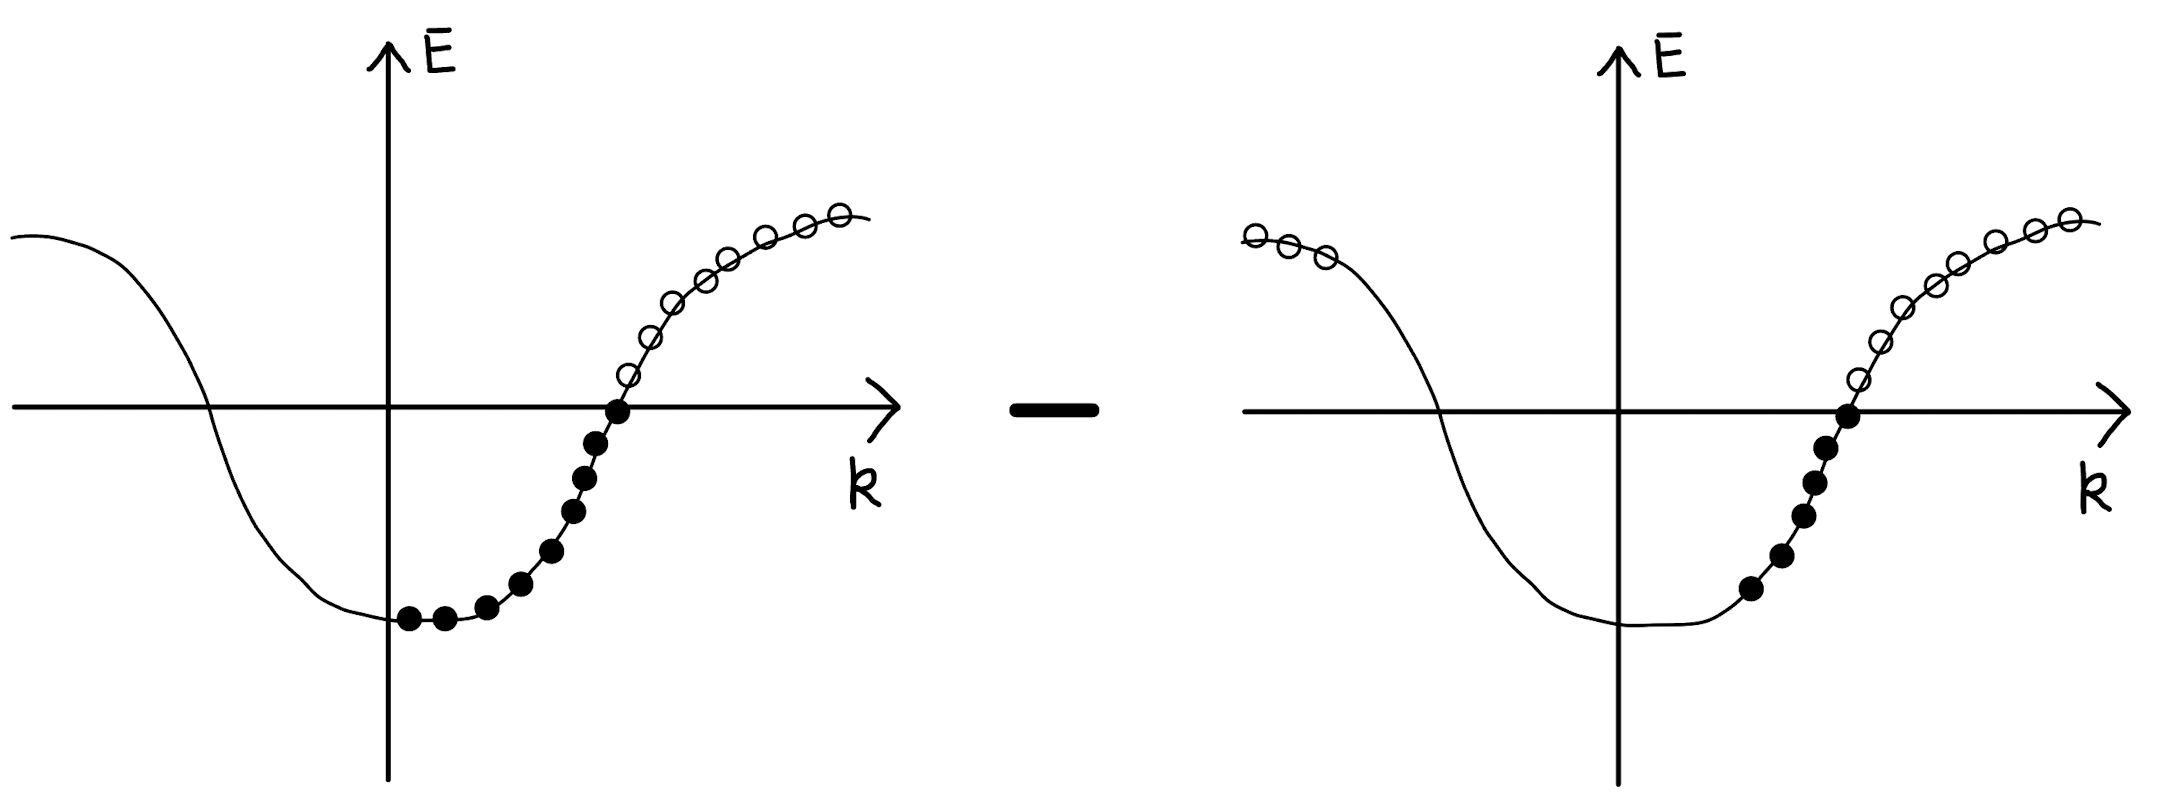
\includegraphics[align=c,width=0.45\linewidth]{pics/LL-k-shift}. \label{eq:inf-subtraction-fig}
\end{equation}
Then the commutator counts the number of modes transported to the left: $[\rho_{k}, \rho_{k}^\dagger] \simeq \frac{kL}{2\pi}$.
The above argument can be equivalently formulated as the normal ordering ${:\mathrel{O}:} \equiv O- \langle 0|O|0\rangle$.
For $k\ne k'$, since $\langle 0|c_k^\dagger c_k|0\rangle=0$, the normal ordering does not affect the result, while for the $k=k'$ case, the normal ordering takes care of the infinity of the particle number operator:
\begin{equation*}
	\sum_q [n_{q} - n_{q+k}]
	= \sum_q \left[{:\mathrel{n_{q}}:} - {:\mathrel{n_{q+k}}:} 
		+ \langle0|n_{q}|0\rangle -\langle0|n_{q+k}|0\rangle \right] 
	= \sum_q [\langle0|n_{q}|0\rangle -\langle0|n_{q+k}|0\rangle].
\end{equation*}
This gives the same result as in (\ref{eq:inf-subtraction-fig}).

We denote the ground state with $N$ fermions as $|0;N\rangle$, which satisfies $\rho_{p>0}|0;N\rangle = \rho^\dagger_{p<0}|0;N\rangle = 0$.
We can thus define a set of canonical bosonic modes (assume $p>0$):
\begin{equation}
	b_p = i \sqrt{\frac{2\pi}{pL}}\rho_p,\ 
	b_p^\dagger = -i\sqrt{\frac{2\pi}{pL}}\rho_p^\dagger, \quad
	[b_q,b_{q'}^\dagger] = \delta_{qq'},\quad
	[\hat N, b_q] = [\hat N, b_q^\dagger] = 0.
\end{equation}
The $N$-particle sector is spanned by the states generated by applying $b_q^\dagger$'s to the ground state.
A general $N$-particle state has the form $|N\rangle = f(\{b_q^\dagger\})|0;N\rangle$.
In order to construct the full Fock space, we also need to include a particle-number-changing operator, the \textit{Klein factor} $\hat F$, that shifts the total number of fermion by one, and commutes with bosonic operator $b_q$:
\begin{equation}
	\left[\hat F, b_q \right] = \left[\hat F, b_q^\dagger \right] = 0, \quad
	\left[\hat F, \hat N \right] = \hat F, \quad 
	\left[\hat F^\dagger, \hat N \right] = -\hat F^\dagger.
\end{equation}
The Klein factor also takes care of the fermionic statistics. 
That is, for the state denoted as $|\{N_i\}\rangle = |N_1,N_2,\cdots,N_m\rangle$.
The Klein factor $\hat F_\eta$ acting on the state will contribute an additional factor
\begin{equation*}
	\hat F_\eta|\{N_i\}\rangle = \exp\left(i\pi\sum_{j=1}^{\eta-1}N_j\right)|N_1,\cdots,N_\eta-1,\cdots,N_m\rangle.
\end{equation*}

Now we try to express the fermion operator $\psi(x) = \frac{1}{\sqrt{L}} \sum_p e^{ipx} c_{p}$
by the bosonic operator set.
First, we consider the commutation relation between the fermion field operator and bosonic mode:
\begin{eqnarray}
	\left[b_q,\psi(x)\right] 
	&=& \frac{i}{\sqrt L}\sqrt{\frac{2\pi}{qL}}\sum_{k}\sum_{p} e^{ipx} [c^\dagger_{k}c_{k+q},c_{p}] 
	= \frac{i}{\sqrt L} \sqrt{\frac{2\pi}{qL}} \sum_{p} e^{ipx} c_{p+q} 
	= +i\sqrt{\frac{2\pi}{qL}} e^{-iqx} \psi(x), \label{eq:bs-comm-1} \\ 
	\left[b_q^\dagger,\psi(x)\right] 
	&=& \frac{-i}{\sqrt L}\sqrt{\frac{2\pi}{qL}}\sum_{k}\sum_{p} e^{ipx} [c^\dagger_{k+q}c_{k},c_{p}] 
	= \frac{-i}{\sqrt L} \sqrt{\frac{2\pi}{qL}} \sum_{p} e^{ipx} c_{p-q} 
	= -i\sqrt{\frac{2\pi}{qL}} e^{+iqx}\psi(x). \label{eq:bs-comm-2}
\end{eqnarray}
We remark here that the fermion field $\psi(x)$ is the linearized band containing all momenta.
We shall not worry about the left mover, which will be regarded as in a different band.

Since $b_q|0;N\rangle=0$ for $q>0$, the commutation relation (\ref{eq:bs-comm-1}) leads to 
\begin{equation*}
	\left[b_{q}, \psi(x)\right]|0;N\rangle = b_{q} \psi(x)|0;N\rangle = i\sqrt{\frac{2\pi}{qL}} e^{-iqx}|0;N\rangle.
\end{equation*}
Thus, $\psi(x)|0;N\rangle$ is an eigenstate of $b_q$, i.e., a coherent state:
\begin{equation*}
	\psi(x)|0;N\rangle
	= \Lambda(x) \hat F \exp\left[i\sum_{q>0} \sqrt{\frac{2\pi}{qL}} b_q^\dagger e^{-iqx}\right]|0;N\rangle,\quad
	\Lambda(x) = \frac{1}{\sqrt L}\sum_k e^{ikx}\ \langle 0;N-1| c_{k,r}|0;N\rangle 
	= \frac{e^{ik_F}}{\sqrt L}.
\end{equation*}
For future convenience, we define
\begin{equation*}
	\varphi(x) = \sum_{q>0} \sqrt{\frac{2\pi}{qL}} b_q e^{iqx},\quad
	\varphi^\dagger(x) = \sum_{q>0} \sqrt{\frac{2\pi}{qL}} b_q^\dagger e^{-iqx}.
\end{equation*}
The commutation relation (\ref{eq:bs-comm-2}) also leads to $\psi(x) b_{q}^{\dagger} =\left(b_{q}^{\dagger}+i\sqrt{\frac{2\pi}{qL}} e^{+iqx}\right) \psi(x)$, which implies
\begin{equation*}
	\psi(x) f\left[\left\{b_{q}^{\dagger}\right\}\right] 
	=f\left[\left\{b_{q}^{\dagger}+i\sqrt{\frac{2\pi}{qL}} e^{+iqx}\right\}\right] \psi(x).
\end{equation*}
Then, for a generic $N$-particle state:
\begin{equation*}
\begin{aligned}
	\psi(x)|N\rangle 
	&= f\left[\left\{b_{q}^{\dagger}+i\sqrt{\frac{2\pi}{qL}} e^{+iqx}\right\}\right] \psi(x)|0;N\rangle
	= f\left[\left\{b_{q}^{\dagger}+i\sqrt{\frac{2\pi}{qL}} e^{+iqx}\right\}\right] \Lambda(x) \hat{F} e^{i\varphi^\dagger(x)}|0;N\rangle \\
	&= \Lambda(x) \hat{F} e^{i\varphi^\dagger(x)} f\left[\left\{b_{q}^{\dagger}+i\sqrt{\frac{2\pi}{qL}} e^{+iqx}\right\}\right]|0;N\rangle 
	= \Lambda(x) \hat{F} e^{i\varphi^\dagger(x)}e^{i\varphi(x)} f\left[b_{q}^{\dagger}\right] e^{-i\varphi(x)}|0;N\rangle \\
	&= \Lambda(x) \hat{F} e^{i\varphi^\dagger(x)} e^{i\varphi(x)}|N\rangle,
\end{aligned}
\end{equation*}
where we have used the BCH formula $e^A B e^{-A} = B + [A,B]$ if $[A,B]$ is a c-number.
The BCH formula also implies $e^{i\varphi^\dagger(x)} e^{i\varphi(x)} = e^{i[\varphi(x)+\varphi^\dagger(x)]}e^{\frac{1}{2}[\varphi(x),\varphi^\dagger(x)]}$, which gives the mapping $\psi(x) \sim \hat{F} e^{i\sqrt{4\pi}\phi(x)}$, where the bosonic field in the operator language is (a regulator controlled by $\alpha$ is introduced)
\begin{equation}
	\phi(x) \equiv \varphi(x)+\varphi^\dagger(x)= \frac{1}{\sqrt{L}} \sum_{q>0} e^{-\alpha q/2} \frac{1}{\sqrt{2q}} \left(b_q e^{iqx} + b_q^\dagger e^{-iqx} \right).
\end{equation}
If we identify $a_q \simeq \sqrt{L}b_q$ (so that their commutation relations agree), we recover the usual bosonic field expansion.
The additional factor comes from the commutator:
\begin{equation*}
\begin{aligned}
	\left[\varphi(x),\varphi^\dagger(x)\right] &= \sum_q \frac{2\pi}{qL} [i b_q^\dagger e^{-iqx-\alpha q/2}, i b_q e^{iqx-\alpha q/2}] 
	= \frac{2\pi}{L} \sum_{q>0} \frac{1}{q} e^{-\alpha q} \\
	&= \sum_n \frac{1}{n}\left\{\exp\left[-\frac{2\pi \alpha}{L}\right]\right\}^n
	= -\ln\left\{ 1-\exp\left[-\frac{2\pi \alpha}{L}\right]\right\},
\end{aligned}
\end{equation*}
The exponential of which is
\begin{equation*}
	e^{\frac{1}{2}\left[\varphi(x),\varphi^\dagger(x)\right]} = \sqrt{\frac{1}{1-\exp\left[-2\pi \alpha/L\right]}}
	\simeq \sqrt{\frac{L}{2\pi \alpha}}.
\end{equation*}
Therefore the final result is $\psi(x) = \hat{F} \frac{1}{\sqrt{2\pi \alpha}} e^{ik_F} e^{i\sqrt{4\pi}\phi(x)}$.
Note that we can shift the momentum so that the Fermi point $k_F = 2\pi N/L$ becomes the origin.
Eq.~(\ref{eq:bosonization}) is then recovered.

For the left mover, the sign convention is slightly different.
We can choose a different definition of $b_p$ for $p<0$:
\begin{equation}
	b_p = -i \sqrt{\frac{2\pi}{pL}}\rho_p,\ 
	b_p^\dagger = i\sqrt{\frac{2\pi}{pL}}\rho_p^\dagger,\quad q<0.
\end{equation}
This sign change corresponds to the convention in Eq.~(\ref{eq:bosonization}).


\subsection{Bosonization dictionary}
We aim to bosonize the interacting Fermion Hamiltonian
\begin{equation*}
	H = H_0 + H_\text{int} = \int dx \left[v_F\psi^\dagger_+(x)(-i\partial_x)\psi_+(x) +v_F\psi_-^\dagger(x)(i\partial_x)\psi_-(x) + u(\psi^\dagger(x)\psi(x))^2 \right].
\end{equation*}
We first consider the free part.
Note the commutation relation $[H_0,b_{q}^\dagger] = |q| b_{q}^\dagger$, so $H_0$ in terms of bosonic operator $b_q$ can only be the bilinear $H_0 = v_F \sum_{q} |q| b^\dagger_q b_q$, which is nothing but the Klein-Gordon Hamiltonian 
\begin{equation}
	H_0 = \frac{v_F}{2} \int dx [\Pi^2+(\partial_x\phi)^2].
\end{equation}

Next, consider the fermion density
\begin{equation*}
	\psi^\dagger(x)\psi(x) = \psi_-^\dagger(x)\psi_-(x) + \psi_+^\dagger(x)\psi_+(x) + e^{-2ik_F x} \psi_+^\dagger(x)\psi_-(x)+e^{2ik_F x}\psi_-^\dagger(x)\psi_+(x).
\end{equation*}
We first consider the bosonization of the fermion bilinear $\psi_+^\dagger(x)\psi_+(x)$.
We will use the point-splitting trick to regulate the infinity: $\psi^\dagger_+(x)\psi_+ \simeq \lim_{\alpha\rightarrow 0} \psi_+^\dagger(x+\alpha)\psi_+(x)$.
Using Eq.~(\ref{eq:normord-id}), 
\begin{equation*}
\begin{aligned}
	\lim_{a\rightarrow 0^+}\psi_+^\dagger(x+a)\psi_+(x)
	&= \lim_{a\rightarrow 0^+}\frac{1}{2\pi \alpha} e^{-i\sqrt{4\pi}\phi_+(x+a)}e^{i\sqrt{4\pi}\phi_+(x)} 
	\simeq \frac{1}{2\pi \alpha} \normord{e^{-i\sqrt{4\pi}\partial_x\phi_+(x)a}} \ e^{4\pi G_+(a)} \\
	&= \lim_{a\rightarrow 0^+}\lim_{\alpha\rightarrow 0^+}\frac{1}{2\pi} \frac{1}{\alpha-ia} \left[1-i\sqrt{4\pi}\partial_x\phi_+(x)a \right]
	\sim \frac{1}{\sqrt\pi} \partial_x\phi_+(x).
\end{aligned}
\end{equation*}
Note that we have omitted the infinity in the above derivation.
Or equivalently, the above mapping can be directly calculated using the bosonization map:
\begin{equation*}
\begin{aligned}
	\normord{\psi_+^\dagger(x)\psi_+(x)}
	&= \frac{1}{L}\sum_{q} {:\mathrel{c_{q}^\dagger c_{q}}:} + \frac{1}{L}\sum_{q>0}[e^{-iqx}\rho^\dagger_{q}+e^{iqx}\rho_{q}]
	= \frac{1}{L}\sum_{q>0} \sqrt\frac{qL}{2\pi} [e^{-iqx}b^\dagger_{q}+e^{iqx}b_{q}] \\
	&\simeq \frac{1}{\sqrt{\pi}} \int_0^\infty \frac{dq}{2\pi} \sqrt\frac{q}{2} \left[e^{iqx}a_{q} - e^{-iqx}a^\dagger_{q}\right] 
	= \frac{1}{\sqrt\pi} \partial_x\phi_+(x).
\end{aligned}
\end{equation*}
Similarly, for the left mover, $\normord{\psi_-^\dagger(x)\psi_-(x)}= \frac{1}{\sqrt\pi} \partial_x\phi_-(x)$.
So the first part of the density is just $\frac{1}{\sqrt\pi}\partial_x\phi(x)$.
We can omit the second part due to its fast oscillation when the system is away from half-filling.
In this case the interaction is just $H_\text{int} = \frac{1}{\pi}\int dx (\partial_x\phi)^2$.
We will then focus on the half-filling case.
To avoid subtlety, we consider the lattice Hamiltonian where the interaction is $H_\text{int} = u \sum_j \left(n_j-\frac{1}{2}\right) \left(n_{j+1}-\frac{1}{2} \right)$.
The bosonization procedure gives:
\begin{equation*}
\begin{aligned}
	H_\text{int} =& \ u \int dx \left[: \psi_+^{\dagger}(x) \psi_+(x)+\psi_-^{\dagger}(x) \psi_-:+(-1)^{j}\left(\psi_+^{\dagger}(x) \psi_-(x)+\psi_-^{\dagger}(x) \psi_+(x)\right)\right] \\
	&\ \times\left[: \psi_+^{\dagger}(x) \psi_+(x)+\psi_-^{\dagger}(x) \psi_-(x):-(-1)^{j}\left(\psi_+^{\dagger}(x) \psi_-(x)+\psi_-^{\dagger}(x) \psi_+(x)\right)\right] \\
	=&\ u\int dx \left[\left(\frac{1}{\sqrt{\pi}} \partial_{x} \phi\right)^{2}-\left(\psi_+^{\dagger} \psi_- + \psi_-^{\dagger} \psi_+\right)^{2} \right] 
		+\left\{(-1)^j\ \text{oscillations} \right\}.
\end{aligned}
\end{equation*}
The second part in the fermion density is
\begin{equation*}
	\psi_+^\dagger \psi_- + h.c.
	= \frac{1}{2\pi a} e^{i\sqrt{4\pi}\phi(x)} + h.c. 
	= \frac{1}{\pi a}\cos\left[\sqrt{4\pi}\phi(x)\right].
\end{equation*}
When squaring it, we should also use the point-splitting to regulate the expression:\footnote{That is why we are so careful about the interaction: the position shift $x\rightarrow x+a$ introduces an additional phase. If naively squared, we will get the wrong sign.}
\begin{equation*}
	\frac{1}{\pi^2 a^2} \cos\left[\sqrt{4\pi}\phi(x)\right]\cos\left[\sqrt{4\pi}\phi(x+a)\right].
\end{equation*}
Using the identity $\cos\alpha \cos\beta = \frac{1}{2}[\cos(\alpha+\beta)+\cos(\alpha-\beta)]$, the square is (also note that any constant can be neglected since the final expression is normal-ordered)
\begin{equation*}
	\frac{1}{2\pi^2 a^2}\left[\cos\left(\sqrt{16\pi}\phi\right)+\cos\left(\sqrt{4\pi}\partial_x\phi \right)\right]
	\simeq \frac{\cos\left[\sqrt{16\pi}\phi(x)\right]}{2\pi^2 a^2} - \frac{[\partial_x\phi(x)]^2}{\pi}.
\end{equation*}
The interaction is then mapped to
\begin{equation}
	H_\text{int} = u\int dx \left\{\frac{2}{\pi}(\partial_x\phi)^2 - \frac{\cos\left[\sqrt{16\pi}\phi(x)\right]}{2\pi^2 a^2}\right\}.
\end{equation}



\section{Luttinger Liquid Theory}

In this section, we consider the 1D half-filling interacting system.
Based on the bosonization dictionary we constructed, the bosonic Hamiltonian is
\begin{equation*}
	H = \int \frac{dx}{K} \left\{ \frac{1}{2}\left[K \Pi^2 + \frac{1}{K}(\partial_x\phi)^2 \right] + \frac{y}{2\pi^2 a^2} \cos\left[\sqrt{16\pi}\phi\right] \right\},\quad
	K = \frac{1}{\sqrt{1+4u/\pi}}, \ y = \frac{u}{\sqrt{1+4u/\pi}}.
\end{equation*}
We can shift the variables as $\Pi \rightarrow \Pi/\sqrt K$, $\phi \rightarrow \sqrt K \phi$,
(note that the canonical commutation relation is preserved in this way) and the Hamiltonian becomes
\begin{equation*}
	H = \int \frac{dx}{K} \left\{ \frac{1}{2}\left[\Pi^2 + (\partial_x\phi)^2 \right] + \frac{y}{2\pi^2 a^2} \cos\left[\sqrt{16\pi K}\phi\right] \right\}.
\end{equation*}
Omit the constant factor, and the Euclidean Lagrangian is
\begin{equation}
	\mathcal L = \frac{1}{2}(\nabla \phi)^2 + \frac{y}{2\pi^2 a^2} \cos\left[\sqrt{16\pi K}\phi\right]
	\equiv \frac{1}{2}(\nabla \phi)^2 + \frac{y}{2\pi^2 a^2} \cos\left[\beta\phi\right].
\end{equation}
This is called the Sine-Gordon model.


\subsection{RG Analysis}
When writing $\phi$ as the sum of slow and fast modes, the partition function is
\begin{equation*}
	Z = \int D\phi_s e^{-\frac{1}{2}\int d^2x (\nabla\phi_s)^2}
	\left\langle\exp\left\{-\frac{y}{2\pi^2 a^2} \int d^2 x \cos\left[\beta(\phi_s+\phi_f)\right] \right\}\right\rangle_f
\end{equation*}
Under the rescaling $x \rightarrow x' = e^{dt} x$, $\phi(x) \rightarrow \phi'(x') = \phi(x')$, the free field action is invariant.
The effective action can be perturbatively evaluated as
\begin{equation*}
	S_{\mathrm{eff}} = S_0 + \langle S_1\rangle_f - \frac{1}{2}(\langle S_1^2\rangle_f - \langle S_1\rangle_f^2) + \text{higher orders}.
\end{equation*}
To the first order, 
\begin{equation*}
	\langle S_1\rangle = \frac{y}{2\pi^2 a^2} \int d^2 x \left\langle\cos\left[\beta(\phi_s+\phi_f)\right] \right\rangle_f 
	= -\frac{y}{2\pi^2 a^2} \int d^2 x \cos(\beta\phi_s)\langle\cos(\beta\phi_f)\rangle_f,
\end{equation*}
where we have used the identity $\cos\left[\beta(\phi_s)\right] = \cos(\beta\phi_s)\cos(\beta\phi_f)-\sin(\beta\phi_s)\sin(\beta\phi_f)$,
and note the fact that $\sin(\beta\phi_f)$ term will not contribute when integrated over the fast field. 
Also, note of the fact that $\langle e^{i\beta\phi}\rangle = e^{-\frac{1}{2}\beta^2 \langle\phi^2\rangle}$.
We then compute the expectation
\begin{equation*}
\begin{aligned}
	\left\langle \cos(\beta\phi)\right\rangle_f
	&= \left\langle \frac{e^{i\beta\phi} + e^{-i\beta\phi}}{2}\right\rangle_f
	= e^{-\frac{1}{2}\beta^2\langle\phi^2\rangle} 
	= \exp\left[-\frac{\beta^2}{2}\int^\Lambda_{\Lambda(1-dt)}\frac{k dk}{2\pi} \frac{1}{k^2} \right] 
	= 1-\frac{\beta^2}{4\pi\Lambda}dt.
\end{aligned}
\end{equation*}
In this way, the rescaling is $y \rightarrow e^{2dt}\left(1-\frac{\beta^2}{4\pi\Lambda}dt\right) y$.
In the cut-off unit where $\Lambda$ is set to $1$, the beta function is
\begin{equation*}
	\frac{dy}{dt} = (2-4K) y = 4\left[\frac{1}{2}-\left(1-\frac{4u}{\pi}\right)^{-\frac{1}{2}}\right]y.
\end{equation*}
Setting $x\equiv 2-4K$, the first-order RG equation is
\begin{equation}
	\frac{dy}{dt} = xy.
\end{equation}

Now consider the second-order expansion
\begin{equation*}
\begin{aligned}
	\delta S^{(2)} 
	=&\ \frac{y^2}{4\pi^4 a^4} \int d^2 x_1 d^2 x_2 \left\{ \left\langle \cos\left[\beta\phi_s(x_1)+\beta\phi_f(x_1)\right] \cos\left[\beta\phi_s(x_2)+\beta\phi_f(x_2)\right] \right\rangle_f \right. \\
	&\ \left. -\left\langle \cos\left[\beta\phi_s(x_1)+\beta\phi_f(x_1)\right]\right\rangle_f \left\langle \cos\left[\beta\phi_s(x_2)+\beta\phi_f(x_2)\right]\right\rangle_f \right\}
\end{aligned}
\end{equation*}
The first term is 
\begin{equation*}
\begin{aligned}
	&\  \cos\left[\beta\phi_s(x_1)+\beta\phi_f(x_1)\right] 
		\cos\left[\beta\phi_s(x_2)+\beta\phi_f(x_2)\right] 
	= \frac{1}{2}\cos\left[\beta\phi(x_1)+\beta\phi(x_2)\right] + 
	  \frac{1}{2}\cos\left[\beta\phi(x_1)-\beta\phi(x_2)\right] \\
	=&\ \frac{1}{2}\left\{\cos\left[\beta\phi_s(x_1)+\beta\phi_s(x_2)\right] \cos\left[\beta\phi_f(x_1)+\beta\phi_f(x_2)\right] + \cos\left[\beta\phi_s(x_1)-\beta\phi_s(x_2)\right] \cos\left[\beta\phi_f(x_1)-\beta\phi_f(x_2)\right] \right\} \\ 
	&+ \text{sin terms}.
\end{aligned}
\end{equation*}
Similarly, we neglect all $\sin(\beta\phi_f)$ terms.
The averaging gives:
\begin{equation*}
\begin{aligned}
	&\  \left\langle\cos\left[\beta\phi_s(x_1)+\beta\phi_f(x_1)\right] 
		\cos\left[\beta\phi_s(x_2)+\beta\phi_f(x_2)\right]\right\rangle_f \\
	=&\ \frac{1}{2} \left\{e^{-\frac{\beta^2}{2}\langle[\phi_f(x_1)+\phi_f(x_2)]^2\rangle} \cos[\beta\phi_s(x_1)+\beta\phi_s(x_2)] + e^{-\frac{\beta^2}{2}\langle[\phi_f(x_1)-\phi_f(x_2)]^2\rangle} \cos[\beta\phi_s(x_1)-\beta\phi_s(x_2)] \right\}.
\end{aligned}
\end{equation*}
For the second term,
\begin{equation*}
\begin{aligned}
	&\ \left\langle \cos\left[\beta\phi_s(x_1)+\beta\phi_f(x_1)\right]\right\rangle_f \left\langle \cos\left[\beta\phi_s(x_2)+\beta\phi_f(x_2)\right]\right\rangle_f 
	=\ \cos[\beta\phi_s(x_1)]\cos[\beta\phi_s(x_2)] e^{-\frac{\beta^2}{2}\langle\phi_f^2(x_1)+\phi_f^2(x_2)\rangle} \\
	=&\ \frac{1}{2}e^{-\beta_f^2 \langle \phi^2\rangle} \left\{ \cos[\beta\phi_s(x_1)+\beta\phi_s(x_2)] + \cos[\beta\phi_s(x_1)-\beta\phi_s(x_2)] \right\}
\end{aligned}
\end{equation*}
The subtraction is
\begin{equation*}
	e^{-\beta^2\langle\phi_f^2\rangle} \left\{
		\left(e^{-\beta^2 \langle\phi_f(x_1)\phi_f(x_2)\rangle}-1 \right)\cos\left[\beta\phi_s(x_1) +\beta\phi_f(x_2)\right] 
	 + \left(e^{\beta^2 \langle\phi_f(x_1)\phi_f(x_2)\rangle}-1 \right)\cos\left[\beta\phi_s(x_1) -\beta\phi_f(x_2)\right] \right\}
\end{equation*}
Consider the bosonic correlation
\begin{equation*}
	\mathcal G(\bm x) \equiv \langle \phi_f(x) \phi_f(0)\rangle_f = F(\bm x) dt + O(dt^2).
\end{equation*}
A straightforward calculation with the hard cut-off yields $F(\bm x)$ a Bessel function with a long oscillating tail.
However, it can be shown that implementing a smooth cut-off will make $F(\bm x)$ short ranged.
For this reason, we can switch to the center-of-mass coordinate: $\bm R = \frac{\bm x_1 + \bm x_2}{2}, \ \bm r = \bm x_1 - \bm x_2$.
In this way, the term $\cos\left[\beta\phi_s(x_1) +\beta\phi_f(x_2)\right]$ is approximated by a $\cos\left[2\beta\phi_s(x)\right]$ term, which is oscillating at double frequency, and thus is regarded as irrelevant.

The remaining term can be simplified by the approximation:
\begin{equation*}
	\cos\left[\beta\phi_s(x_1) -\beta\phi_f(x_2)\right]
	\sim 1-\frac{\beta^2}{2} [\bm r \cdot \nabla\phi_s(\bm R)]^2
\end{equation*}
The constant term only contributes to the infinity of free energy.
The non-trivial contribution is:
\begin{equation*}
	\int d^2 R \int d^2 r \left(e^{\beta^2 \langle\phi_f(x_1)\phi_f(x_2)\rangle}-1 \right)\cos\left[\beta\phi_s(x_1) -\beta\phi_f(x_2)\right] 
	\simeq  -\frac{\beta^4}{2} \int d^2 R \int d^2r F(\bm r) [\bm r \cdot \nabla\phi_s(\bm R)]^2.
\end{equation*}
Note that $\int d^2r\ r_i r_j = \delta_{ij} \int r dr d\theta\ r^2 \cos^2(\theta) = \pi \delta_{ij} \int dr\ r^3$, and the above expression can be formulated as:
\begin{equation*}
\begin{aligned}
	&\ \int d^2 R \int d^2 r \left(e^{\beta^2 \langle\phi_f(x_1)\phi_f(x_2)\rangle}-1 \right)\cos\left[\beta\phi_s(x_1) -\beta\phi_f(x_2)\right] \\
	\simeq &\ -\frac{\pi \beta^4}{2} \left[\int_0^\infty dr\ r^3 F(r)\right] \int d^2 R [\nabla\phi_s(\bm R)]^2 
	\equiv  -\pi \beta^4 A \times \frac{1}{2}\int d^2 R [\nabla\phi(\bm R)]^2.
\end{aligned}
\end{equation*}
We see the second-order perturbation renormalize the free field, as it change the normalization of the field:
\begin{equation*}
	\phi \rightarrow \phi' = Z^{\frac{1}{2}} \phi, \quad 
	Z^{\frac{1}{2}} = 1 +\frac{1}{2} \pi \beta^4 A \left( \frac{y}{2\pi^2 a^2} \right)^2.
\end{equation*}
To preserve the form of the $\cos\beta\phi$ term, we have to shift $d\beta = Z^{-\frac{1}{2}}\beta - \beta = -\frac{\beta^5 A}{8 \pi^3 a^4} y^2 dt$.
The RG equation to the second order is then
\begin{equation*}
	\frac{dx}{dt} = \frac{d}{dt}\left(2-\frac{\beta^2}{4\pi}\right)
	= \frac{\beta^6 A}{16\pi^4 a^4} y^2.
\end{equation*}
The $\beta = \sqrt{4\pi(2-x)}$ is dependent on $x$.
While near the fixed point $x=y=0$, $\beta \simeq \sqrt{8\pi}$, the RG equation is then
\begin{equation}
	\frac{dy}{dt} = xy, \quad
	\frac{dx}{dt} = \frac{32 A}{\pi a^4} y^2.
\end{equation}
Setting $c^2 = 32A/\pi a^4$, we note that the differential relation implies $d(x^2- c^2 y^2) = 0$, i.e., the flow is along the hyperbolas, with a marginal line described by $x = \pm cy$.
The RG flow is shown in the following:
\begin{equation*}
	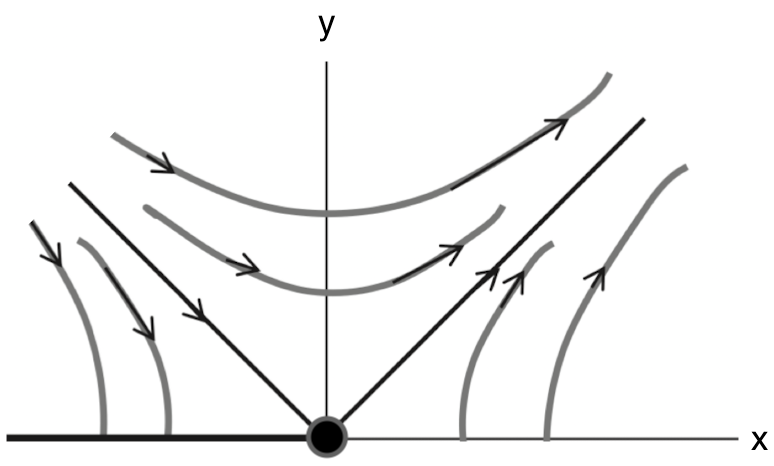
\includegraphics[hsmash=c,width=0.2\linewidth]{pics/LL-RG-flow}
\end{equation*}
We see that there are three regimes of the RG flow: in the weak interacting regime, the field theory flows to the Tomonaga-Luttinger (TL) line; for strong interaction, depending on the sign of $y$, the systems develop two charge-density-wave (CDW) order, namely the Neel-CDW, and Peierls-CDW.


\subsection{Phase Diagram}

\subsubsection{Tomonaga-Luttinger Liquid}
When $K<\frac{1}{2}$, the interacting cosine term become irrelevant.
In this case, the system is in a liquid state, called the \textit{Tomonaga-Luttinger liquid}.
The system on the TL line is described by the non-interacting Hamiltonian:
\begin{equation}
	H = \int \frac{dx}{K} \frac{1}{2}\left[K \Pi^2 + \frac{1}{K}(\partial_x\phi)^2 \right],
\end{equation}
As discussed, we can define a new set of variables to map the Hamiltonian to that of the original bosonic model:
\begin{equation}
\begin{aligned}
	\phi' &= \frac{\phi'_-+\phi'_+}{\sqrt 2} = \frac{\phi}{\sqrt{K}} = \frac{\phi_-+\phi_+}{\sqrt{2K}}, \\
	\theta' &= \frac{\phi'_--\phi'_+}{\sqrt 2} = \sqrt{K} \theta = \sqrt{\frac{K}{2}}(\phi_--\phi_+).
\end{aligned}
\end{equation}
The fermion mode is
\begin{equation}
	\psi_{\pm}(x) = \frac{1}{\sqrt{2\pi a}} \exp\left[-i\sqrt{2\pi} \phi'_{\pm}(x) \right]
	= \frac{1}{\sqrt{2\pi a}} \exp\left\{-i\sqrt{2\pi} \left[K_\pm \phi_+(x)+ K_\mp \phi_-(x) \right]\right\},
\end{equation}
where 
\begin{equation}
	K_\pm \equiv \frac{K^{\frac{1}{2}} \pm K^{-\frac{1}{2}}}{2}.
\end{equation}
The Greens function is (assume $\tau>0$):
\begin{equation}
	-G_{\pm}(x,\tau) 
	= \frac{1}{2\pi a} e^{2\pi \langle \phi'_\pm(x,\tau)\phi'_\pm(0) - \phi'_\pm(0)\phi'_\pm(0) \rangle}
\end{equation}
The bosonic correlation is
\begin{equation}
	\langle \phi'_\pm(x,\tau)\phi'_\pm(0) \rangle
	= K_\pm^2 \langle \phi_+(x,\tau)\phi_+(0)\rangle + K_\mp^2 \langle\phi_-(x,\tau)\phi_-(0)\rangle 
	= \frac{K_\pm^2}{2\pi}\ln \frac{L/2\pi}{a-ix+\tau} + \frac{K_\mp^2}{2\pi}\ln \frac{L/2\pi}{a+ix +\tau}.
\end{equation}
So that
\begin{equation}
	-G_{\pm}(x,\tau) 
	= \frac{1}{2\pi a} \left[\frac{a}{a + \tau - ix}\right]^{K_\pm^2} \left[\frac{a}{a + \tau + i x}\right]^{K_\mp^2} 
	= \frac{1}{2\pi} \frac{1}{a + \tau \mp ix} \left[\frac{a^2}{a^2+x^2+\tau^2}\right]^{K_-^2}.
\end{equation}
Note that when $K=0$, $K_-=0$, and the theory agrees with the free fermion prediction:
\begin{equation}
	-G(x, 0^+) = \frac{1}{2\pi} \frac{1}{a-ix}
	= \int \frac{dk}{2\pi} e^{ikx-ak} \theta(k)
\end{equation}
However, when $K_- \ne 0$, the additional factor will smear the pole to a brach cut. 
To see this, note that from the dimensional analysis, the Green's function is of anomalous dimension $-K_-^2$.
In the momentum space, this means that the Green's function scales as
\begin{equation}
	G(k,\omega) \sim (k,\omega)^{K_-^2}.
\end{equation}
This implies that the density 
\begin{equation}
	n(k) = n_0 + c k^{K_-^2}.
\end{equation}


\subsubsection{Charge Density Wave Order}
We first consider the case where $y>0$ is sufficiently large. 
Consider
\begin{equation}
	\cos\left[\sqrt{16\pi}\phi(x)\right] = \frac{1}{2} - \sin^2\left[\sqrt{4\pi}\phi(x)\right].
\end{equation}
The energy is minimized if 
\begin{equation}
	\sin\left[\sqrt{4\pi}\phi(x)\right] = \pm 1.
\end{equation}
Note that in our bosonization dictionary,
\begin{equation}
	\psi_{\pm}^\dagger(x)\psi_{\mp}(x) = \frac{1}{2\pi a} e^{\pm i\sqrt{4\pi}\phi(x)},
\end{equation}
so that
\begin{equation}
	\frac{i}{\pi a} \sin\left[\sqrt{4\pi}\phi(x)\right] = \psi_{+}^\dagger(x)\psi_{-}(x)-\psi_{-}^\dagger(x)\psi_{+}(x).
\end{equation}
We know for the Neel-CDW phase, the order parameter is
\begin{equation}
	i\left\langle \psi_{+}^\dagger(x)\psi_{-}(x)-\psi_{-}^\dagger(x)\psi_{+}(x) \right\rangle.
\end{equation}

On the other hand, for $y<0$, consider
\begin{equation}
	\cos\left[\sqrt{16\pi}\phi(x)\right] = -\frac{1}{2} + \cos^2\left[\sqrt{4\pi}\phi(x)\right].
\end{equation}
The energy is minimized if 
\begin{equation}
	\cos\left[\sqrt{4\pi}\phi(x)\right] = \pm 1.
\end{equation}




\subsection{One-dimensional Hubbard Model}
Now we consider the fermion with spin.
The Hubbard model has a non-interacting part,
\begin{equation}
	H_{0}=-\frac{1}{2} \sum_{s, n}\left[\psi_{s}^{\dagger}(n) \psi_{s}(n+1)+\text { h.c. }\right]+\mu \sum_{s, n} \psi_{s}^{\dagger}(n) \psi_{s}(n),
\end{equation}
where $s=\uparrow, \downarrow$ are two possible spin orientations. We do not assume $k_F = \frac{\pi}{2}$ at this point, and use a general chemical potential $\mu$.
Following the usual route, we get two copies of the spinless model:
\begin{equation}
	H_{0}=\sum_{s} \int \frac{d k}{2 \pi} (\mu-\cos k) \psi_{s}^{\dagger}(k) \psi_{s}(k),
\end{equation}
and the continuum version:
\begin{equation}
\begin{aligned}
	H_0 &= v_F \sum_{s} \int d x \left[
		\psi_{s+}^{\dagger}(x)\left(-i \partial_{x}\right) \psi_{s+}(x) +
		\psi_{s-}^{\dagger}(x)\left( i \partial_{x}\right) \psi_{s-}(x)
	\right] \\
	&= \frac{v_F}{2} \sum_s \int d x \left[\Pi_{s}^{2}+\left(\partial_x \phi_{s}\right)^{2}\right].
\end{aligned}
\end{equation}
Let us now turn on the Hubbard interaction,
\begin{equation}
	H_{\mathrm{int}}=U \sum_{n} \psi_{\uparrow}^{\dagger}(n) \psi_{\uparrow}(n) \psi_{\downarrow}^{\dagger}(n) \psi_{\downarrow}(n),
\end{equation}
where $\psi_{\uparrow}, \psi_{\downarrow}$ stand for the original non-relativistic fermion. 
The Hubbard interaction is just the extreme short-range version of the screened Coulomb potential between fermions. 
Due to the Pauli principle, only opposite-spin electrons can occupy the same site.

Let us now express this interaction in terms of the Dirac fields:
\begin{equation}
	\psi_{\uparrow}^{\dagger}  \psi_{\uparrow} \psi_{\downarrow}^{\dagger} \psi_{\downarrow} 
	= \left[\psi_{\uparrow+}^{\dagger} \psi_{\uparrow+}+\psi_{\uparrow-}^{\dagger} \psi_{\uparrow-}+
	\left(\psi_{\uparrow+}^{\dagger} \psi_{\uparrow-} e^{-2 i K_{\mathrm{F}} n}+\text{h.c.}\right)\right] 
	\times(\uparrow \rightarrow \downarrow).
\end{equation}
If we expand out the products and keep only the parts with no rapidly oscillating factors, we will, for generic $k_F$, get the following terms:
\begin{equation}
	H_{\mathrm{int}} = U\left(j_{0 \uparrow} j_{0 \downarrow}\right) + U\sum_n \left(\psi_{\uparrow+}^{\dagger}(n) \psi_{\uparrow-}(n) \psi_{\downarrow-}^{\dagger}(n) \psi_{\downarrow+}(n)+\text{h.c.}\right),
\end{equation}
where
\begin{equation}
	U\left(j_{0 \uparrow} j_{0 \downarrow}\right)
	= \sum_n \left(\psi_{\uparrow+}^{\dagger} \psi_{\uparrow+}+\psi_{\uparrow-}^{\dagger} \psi_{\uparrow-}\right)\left(\psi_{\downarrow+}^{\dagger} \psi_{\downarrow+}+\psi_{\downarrow-}^{\dagger} \psi_{\downarrow-}\right)
\end{equation}
If we now bosonize these terms as per the dictionary, we get, in the continuum,
\begin{equation}
	H_{\mathrm{int}} = U\left[\frac{\partial_x \phi_{\uparrow} \partial_x \phi_{\downarrow}}{\pi}+\frac{1}{2\pi^{2} \alpha^{2}} \cos \sqrt{4 \pi}\left(\phi_{\uparrow}-\phi_{\downarrow}\right)\right]
\end{equation}
We can now separate the theory into two parts by introducing charge and spin fields $\phi_{c}$ and $\phi_{s}$:
\begin{equation}
	\phi_{c/s}=\frac{\phi_{\uparrow} \pm \phi_{\downarrow}}{\sqrt{2}}.
\end{equation}
The parametrization bring the first term in the interaction to a free theory:
\begin{equation}
\begin{aligned}
	\partial_x \phi_{\uparrow} \partial_x \phi_{\downarrow}
	&= \frac{1}{2} \partial_x (\phi_{c}+\phi_s) \partial_x (\phi_c-\phi_s) \\
	&= \frac{1}{2} \left[(\partial_x \phi_c)^2 + (\partial_x \phi_s)^2\right].
\end{aligned}
\end{equation}
The Hamiltonian then become decoupled:
\begin{equation}
	H =H_{c}+H_{s},
\end{equation}
where the charge and spin part of the Hamiltonian are:
\begin{equation}
\begin{aligned}
	H_{c} &=\int \frac{dx}{2 K_c}\left[K_{c} \Pi_{c}^{2}+\frac{1}{K_{c}}\left(\partial \phi_{c}\right)^{2}\right], \\
	H_{s} &=\int \frac{dx}{2 K_s} \left[K_{s} \Pi_{s}^{2}+\frac{1}{K_{s}}\left(\partial \phi_{s}\right)^{2}+\frac{U}{2 \pi^{2} \alpha^{2}} \cos \sqrt{8 \pi} \phi_{s}\right],
\end{aligned}
\end{equation}
where 
\begin{equation}
	K_{c / s} =\frac{1}{\sqrt{1 \pm \frac{U}{\pi}}}.
\end{equation}
The fact that $K_{s} \neq K_{c}$ means that charge and spin move at different velocities. 
This \textit{spin-charge separation} cannot be understood in terms of interacting electrons whose charge and spin would be irrevocably bound. 
This is more evidence of the demise of the quasiparticle, adiabatically connected to the primordial fermion.





\end{document}


             